\documentclass{article}
\usepackage{tikz}
\begin{document}
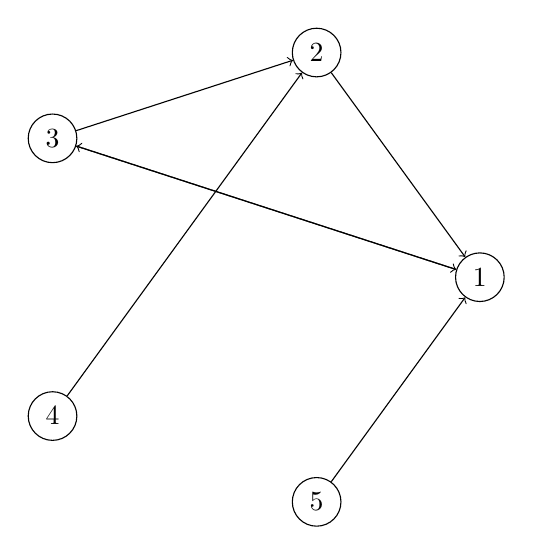
\begin{tikzpicture}[->,node distance=2cm]
\tikzstyle{every node}=[circle,draw]
\node (1) at (3.0,0.0) {1};
\node (2) at (0.9270509831248424,2.8531695488854605) {2};
\node (3) at (-2.427050983124842,1.7633557568774196) {3};
\node (4) at (-2.427050983124843,-1.7633557568774192) {4};
\node (5) at (0.9270509831248417,-2.853169548885461) {5};
\draw[->] (1) -- (3);
\draw[->] (2) -- (1);
\draw[->] (3) -- (1);
\draw[->] (3) -- (2);
\draw[->] (4) -- (2);
\draw[->] (5) -- (1);
\end{tikzpicture}
\end{document}
